\chapter{Solving the Shortest Path Problem}
\label{chap:solvingspp}

Over the years,
various algorithms have been developed 
to address the problem of finding the shortest path in different situations.
In this chapter,
notations and definitions for the shortest path problem is stated first, 
the theory for solving the shortest path problem is described next,
algorithms that are applicable for road networks are then summarised,
including the discussion of their advantages and drawbacks.

\todo[inline]{Big O analysis for all algorithms}
\todo[inline]{Need to talk about results, what should the reader pay attention to? What should they conclude?}
\todo[inline]{assume a path always exist between an OD pair}

\section{Notations and Definitions}
The Shortest Path Problem (SPP) is the problem of finding the shortest path from a given origin  to some destination.
There are two types of SPP hat are going to
be analysed in this chapter:
a single-source and a point to point SPP.  
The Frank-Wolfe algorithm in the TA involves
solving the single-source SPP by finding of shortest path going from one origin to every other destinations the network.
The Path Equilibration method in the TA
Solving the point to point SPP solves from one origin to a specific destination and is used in the Path Equilibration method. 

Using notations from \citet{Klunder} and in the context
of transportation networks,
we denote $ \mathcal{G} = ( \mathcal{V}, \mathcal{A} ) $ for a directed graph,
where $ \mathcal{V} $ denotes the set of nodes (origins, destinations, and intersections)
and $ \mathcal{A} $ the set of arcs (roads);
we say $ \mathcal{A} $ is a subset of the set $ \{ (u, v)\, | \, u, v \in \mathcal{V} \} $ of all ordered pairs of nodes.
We denote the cardinality of $ \mathcal{V} $ be V and $ \mathcal{A} $ be A.
We assume that $ 1 \leq V < \infty $ and $ 0 \leq A < \infty $,
and that a function $ c : \mathcal{A} \rightarrow \mathbb{R} $ is given that assigns a cost (travel time) to any arc $ (u,v) \in \mathcal{A} $.
We write the costs of arc $(u, v)$ as: $ c((u, v)) = c_{uv} $.

The path $\mathcal{P}$ inside a transportation network has to be a directed simple path, 
which is a sequence of nodes and arcs $ (u_1, (u_1, u_2), u_2, \cdots , (u_{k-1}, u_k), u_k ) $
such that $ (u_i, u_{i+1}) \in \mathcal{A}$ for $i = 1,\cdots,k-1$ and $u_i \neq u_j$ for all $ 1 \leq i < j \leq k$.
Note $u_1$ is the origin and $u_k$ is the destination of the path $\mathcal{P}$, $u_1$ and $u_k$ together is called an O-D pair for this path.
%Finally we denote cost of the whole path $C(P) := \sum_{(u,v)\in P} c_{vw}$.

In a transportation network,
the origins and destinations are often called centroids or zones.
They are traffic analysis zones for generating trip demands and supplies
and hold information such as household income and employment information,
these information helps the understanding of trips that are produced and attracted within the zone.
The zones are conceptual nodes in the network and are untravellable,
which means a path between two zone nodes must not contain another zone node.
\todo[inline]{Maybe a picture of the network explain what the zones are.}

When solving SPP for a normal road network,
different measurements such as distance and travel exist for the road length.
But in traffic assignment,
the road length is measured in a nonlinear monotonic increasing travel time function,
encapsulating information such as traffic flow, road capacity and travel speed.
This travel time function is always non-negative so taking advantage of this helps the selection of better algorithms that uses this property.

\begin{comment}
\section{Data Structures}
A Data structure is a way for computers to store, update and manipulate intermediate results.
A good data structure can efficiently speed up the access of the stored data,
which means the performance of solving our shortest path problem does not only depend on the algorithm it self but also the data structure.
In this project,
two data structures are combined to improve the solving speed:
\todo{idea of a data structure is unclear}
\begin{itemize}
    %\item Forward Star (for the label correcting algorithm in Section~\ref{section:labelcorrectingalgorithm}),
    %\item Heap (for the label setting algorithms in Section~\ref{section:labelsettingalgorithm} and onwards).
\end{itemize}
\end{comment}

\begin{comment}
\subsection{Forward Star}\label{chap:forwardstar}
%There is one common characteristic for all of the shortest path algorithms that is going to be discussed in Section~\ref{chapter:solvingspp}:
all arcs emanating from a given node need to be accessed.
An efficient way of visiting every node inside a network and access all their emanating arcs is to use the Forward Star data structure.
The advantage of using this data structure for storing the network is that
the time complexity for finding any node in the network and iterating through all the emanating arcs is $O(1)$.
The exact implementation of Forward Star is not going to be detailed in this report,
but the information can be found in Chapter 5.3 of Urban Transportation Networks \citep{Sheffi}.
This data structure has already been implemented by the second supervisor.
\end{comment}


\section{Generic Shortest Path Algorithm (GSP)}

\todo[inline]{state SPP from node $s$ to node $t$}
\todo[inline]{explain pivot node}
A family of algorithms exist for solving SPP,
in this section we describe the generic case for these
algorithms.

All of these algorithms aim at finding a 
vector ($d_1, d_2,\dots d_v$) of distance labels and its corresponding shortest path \citep{Klunder}.
Each $d_v$ keeps the least distance of any path going from $s$ to $v$, $d_v = \infty$ if no paths has been found.
A shortest path is optimal when it satisfies the following conditions:
\begin{align}
    d_v \leq d_u + c_{uv}, \quad \forall(u,v) \in \mathcal{A}, \label{eq:Bellman1}\\
    d_v  =   d_u + c_{uv}, \quad \forall(u,v) \in \mathcal{P}.
\end{align}
\todo[noline]{what is $\mathcal{P}$?}
The inequalities~(\ref{eq:Bellman1}) is called Bellman's conditions \citep{Bellman}.
In other words,
we wish to find a label vector $d$ which satisfies Bellman's conditions for all of the vertices in the graph.
To maintain the label vector, the algorithm uses a candidate list $\mathcal{Q}$ to store the label distances.

In the label vector,
a node is said to be unvisited when $d_u = \infty$,
scanned when $d_u \neq \infty$ and is still in the candidate list,
and labelled when the node has been retrieved from the candidate list and its distance label cannot be updated further.
\todo[inline]{this means it is guaranteed to represent the minimal distance from $s$ to $t$}

In the generic shortest path algorithm,
we start by putting the origin node in the queue,
and then iteratively find the arc that violates the Bellman's condition (i.e., $d_v > d_u + c_{uv}$),
distance labels are set to a value which satisfies condition (\ref{eq:Bellman1}) to the corresponding node of that arc.
Shortest path going from $s$ to all other nodes in $\mathcal{V}$ is found when (\ref{eq:Bellman1}) is satisfied for all arcs in $\mathcal{A}$.
It may not be obvious but negative costs are permitted in the GSP but not negative cost cycles.

We use $p_u$ to denote the predecessor of node $u$;
shortest path can be constructed by following the predecessor of destination node $t$ back to origin node $s$.

\todo[inline]{diagram showing $u, v, c_{vw}$ etc.}

Algorithm~\ref{algo:gsp} describes the generic shortest path algorithm mentioned above,
with an extra constraint required when solving a TA problem: travelling through zone nodes are not allowed.
\begin{algorithm}
    \caption{The Generic Shortest Path Algorithm \citep{Klunder}}
    \label{algo:gsp}
    \begin{algorithmic}[1]
        \Procedure{GenericShortestPath}{$s$}
        \State $\mathcal{Q} \gets \mathcal{Q} \cup \{s\}$ \Comment{initialisation}
        \State $p_s \gets -1$ \Comment{origin has no predecessor}
        \State $d_s \gets 0$
        \ForAll {$ u \in \mathcal{V} : u \neq s $} \Comment{all nodes are unvisited except the source}
        \State $d_u \gets \infty$
    \EndFor

    \While{ $\mathcal{Q} \neq \emptyset$ }
    \State $ u \gets \text{top}(\mathcal{Q}) $ 
    \State $ u \gets \mathcal{Q} \setminus \{u\} $
    \If{ $u \neq \text{zone} $}
    \ForAll {$v : (u, v) \in \mathcal{A}$} \Comment{for all outgoing arcs from $u$}
    \If {$d_u + c_{vw} < d_v$}
    \State $d_v \gets d_u + c_{vw}$
    \State $p_v \gets u$
    \If {$v \notin \mathcal{Q}$} \Comment{add node $v$ to queue if it is unvisited}
    \State $\mathcal{Q} \gets \mathcal{Q} \cup \{v\}$
\EndIf
                    \EndIf
                \EndFor
            \EndIf
        \EndWhile
    \EndProcedure
\end{algorithmic}
\end{algorithm}

Note GSP is the generic case for a family of algorithms
that use different implementations of the candidate queue $\mathcal{Q}$ \citep{mplomer},
of which solve either the one-source or the point-to-point shortest path problem.

\section{Label Correcting Algorithm}
\todo[inline]{pseudo code}
\label{section:labelcorrectingalgorithm}
The GSP is addressed as a label correcting algorithm when the candidate list is changed to
a first in first out (FIFO) queue.
\todo{Check if its FIFO or double ended queue}
Given the arc costs can be negative (no negative cycle),
and in order to satisfy the Bellman's conditions for all arcs,
the algorithm has to scan all arcs in $\mathcal{A}$ $V-1$ (number of nodes-1) times,
giving a time complexity of $O(mn)$.

In this algorithm,
the distance labels do not get permanently labelled when a pivot node is retrieved from the queue,
another node may `correct' this node's distance label again,
thus the name label correcting algorithm.
This algorithm is also called the Bellman–Ford–Moore algorithm credited to Bellman, Ford and Moore \citep{Bellman,Ford, Moore}.

\section{Label Setting Algorithm}
\label{section:labelsettingalgorithm}
The classical algorithm for solving the single-source shortest path problem is the Label Setting Dijkstra's algorithm.
\todo{say Dijkstra discovered this}
Conceptually the algorithm grows a shortest path tree from the source node radially outward.
The algorithm is said to be label setting as when the pivot node is retrieved from the queue,
the node gets permanently labelled,
the shortest path going to this node is then solved,
the distance label on this pivot node gives the length of the shortest path.
In order to do this, 
the priority queue is modified to always have the minimum distance label in front of the queue.
Hence the algorithm will iterate through all successive pivot nodes exactly once,
labelling pivot nodes in the order of non-decreasing distance labels.

The advantage of this algorithm over the label correcting algorithm is
that all nodes are only visited once,
and the shortest path tree grows outward radially.
Combining these two feature,
it is clear that when the pivot node is the destination node and is 
labelled,
we can stop the algorithm for the point to point SPP case,
which is desirable for the Path Equilibration method.
Algorithm~\ref{algo:p2pdijkstra} shows the Dijkstra's algorithm where the algorithm can be terminated in line 10.

\begin{algorithm}
    \caption{Point to Point Label Setting Algorithm (Dijkstra)}
    \label{algo:p2pdijkstra}
    \begin{algorithmic}[1]
        \Procedure{Dijkstra}{$s, t$}
        \State $\mathcal{Q} \gets \{s\}$ \Comment{initialisation}
        \State $p_s \gets -1$
        \State $d_s \gets 0$
        \ForAll {$ u \in \mathcal{V} : u \neq s $} \Comment{all nodes are unvisited except the source}
        \State $d_u \gets \infty$
    \EndFor

    \While{ $\mathcal{Q} \neq \emptyset$ }
    \State $ u \gets \text{top}(Q) $\Comment{get the node with the minimum distance label}
    \State $ \mathcal{Q} \gets \mathcal{Q} \char`\\ \{u\} $
    \If{ $u = t$ }
    \State \text{Terminate Procedure}
\EndIf
\If{ $u \neq \text{zone} $}
\ForAll {$v : (u, v) \in \mathcal{A}$} \Comment{For all outgoing arcs from $u$}
\If {$d_u + c_{vw} < d_v$}
\State $d_v \gets d_u + c_{vw}$
\State $p_v \gets u$
                        %\If {$v \notin \mathcal{Q}$} \Comment{Include node $v$ if unvisited}
\State $\mathcal{Q} \gets \mathcal{Q} \cup \{v\}$
                        %\EndIf
                    \EndIf
                \EndFor
            \EndIf
        \EndWhile
    \EndProcedure
\end{algorithmic}
\end{algorithm}
Note a path will not be found if the queue becomes empty,
but this stopping condition is safe because we known a path
always exist between an OD pair.

\subsection{Priority Queue and Heap}
\todo[inline]{how do you deal with one node is STL multiple times}
A priority queue is a data structure which sorts elements by their priority,
element with high priority is always retrieved first before an element with a lower priority.
\begin{comment}
In section~\ref{section:labelsettingalgorithm} and on wards,
a specific implementation of the priority queue is used:
min-heap tree (of which also have different types of implementation).
\end{comment}
The idea of the min-heap tree is that the values of a parent node
is always less or equal to its parent node,
by maintaining this property,
the minimum valued element will always be on top,
and retrieving it has only $O(1)$ time complexity.
And for other operations such as adding, removing and updating a node in the heap is at most $O(\log(N))$.
So the heap data structure is very efficient at constantly adding a element and finding the current minimum value.

\subsection{Heap Implementation}
\todo[inline]{explain how this relates to previous results (one is STL and one is Boost, need to be much clearer}

Various implementations of the Heap data structure exist,
with each implementation have some advantages than the other,
for example faster tree balancing, faster push or pop.
\todo{what are these procedures?}

We examine 6 different Heap implementations from the C++ Boost Heap Library \citep{BoostHeap}:
\begin{table}[H]
    \centering
    \begin{tabular}{cccccc}
        & top() & push()    & pop()     & increase() & decrease() \\
        d-ary (Binary)  & O(1)  & O(log(N)) & O(log(N)) & O(log(N))  & O(log(N))  \\
        d-ary (Ternary) & O(1)  & O(log(N)) & O(log(N)) & O(log(N))  & O(log(N))  \\
        Binomial        & O(1)  & O(log(N)) & O(log(N)) & O(log(N))  & O(log(N))  \\
        Fibonacci       & O(1)  & O(1)      & O(log(N)) & O(1)       & O(log(N))  \\
        Pairing         & O(1)  & O($2^{2*\log(\log(N))}$) & O(log(N)) & O($2^{2*\log(\log(N))}$) & O($2^{2*\log(\log(N))}$) \\
        Skew            & O(1)  & O(log(N)) & O(log(N)) & O(log(N)) & O(log(N))   
    \end{tabular}
    \caption{C++ Boost Heap Implementations with Comparison of Amortized Complexity}
    \label{table:heaps}
\end{table}
Where N is the number of elements in the Heap tree, and all time complexities are measured in amortized time,
i.e.\ the average run time if the operation is run for a long period of time,
average out worse case and best case.

We are interested in using these Heap data structures rather than the standard STL priority queue is because of one reason:
the decrease (or increase) function.
The decrease (or increase) function is referred as the decrease-key (or increase-key) operation,
which updates the value of the key in the Heap tree.
Decrease-key is used for a min-heap and increase-key for a max-heap tree.
For the Dijkstra's algorithm,
often nodes are scanned multiple times in the label updating step,
instead of adding the node again into the Heap tree,
we can use decrease-key on the node,
updating its distance label.
This means we can reduce the size of the Heap tree and run time by using decrease-key
rather than adding the same node with different distance label in the queue again.

\begin{comment}
Thus we change Step 2 of the GSP
\begin{verbatim}
Step 2: Label update
if u is not a zone node then
for each outgoing arc (u,v) \in \mathcal{A} do
if d_u + c_{uv} < d_v then
d_v := du + c_{uv}
p_v := u
if v \notin Q then
add v to Q
else
decrease-key(v)
end if
end for
end if
\end{verbatim}
\end{comment}

In table~\ref{table:heaps},
we can observe the Fibonacci Heap has a very interesting time complexity,
constant amortized time for the push, pop and increase-key operation time.
But the fact is,
we do not know how much constant time it really uses.
This also applies to all the other operations.
And since we do not know the time constant for all the operations,
and with different sparsity of the networks,
we need to experiment with all of them.
\todo[inline]{more details about Fibonacci, why good in theory not in practice}

C++ Boost Library Heaps are implemented as max-heaps,
which means in order to use the Fibonacci O(1) increase-key function,
we need to negate the distance labels when we add them into the Heap

All of these run times are slower than the STL version of the Heap.
Upon inspection,
it is found that the increase-key operation is used about between 5\% to 10\%
of the time,
\todo{not actual count yet}
which means the graphs are not dense enough for these Heap structures to outperform a
simple array based priority queue.

\section{Bidirectional Dijkstra}
\section{A* Algorithm}
\todo[inline]{describe in LP sense, solving the dual, potentials etc.}
Up until now,
the Dijkstra's algorithm does not take into account the location of the destination,
the shortest path tree is grown out radially until the destination is labelled.
In a traditional graph where actual distances are used for the distance labels,
a heuristic can be used to direct the shortest path tree to grow toward the destination.
If the heuristic estimate is the distance from each node to the destination,
and the estimate is smaller than or equal to the actual distance going to that destination,
then a shortest path can be found. This is called A* search.
Formally we define the following: Let $h_v$ be a heuristic estimate from node $v$ to $t$,
\todo{potential instead of heuristic?}
we apply Bellman's condition such that an optimal solution exist, that is 
$ h_v \leq h_u + c_{uv}, \quad \forall(u,v) \in \mathcal{A} $.
In other words, the heuristic estimate for each node need to always under estimate the actual distance going from the node to the destination.
\todo[inline]{comment on gurantee of optimal shortest path}

It is proven using geographical coordinates and Euclidean distance as the heuristic estimate,
\todo{reference!}
A* search is guaranteed to work with a huge run time speed up by scanning very few nodes.

In our Path Equilibration method,
we can no longer use geographical coordinates and euclidean distance for the heuristic estimate,
this is because we use travel times as the distances for the arcs.
Although distance is included in the calculation,
we cannot guarantee it to under estimate the travel times.
\todo[inline]{could we use Euclidea distance * min speed ?}

By analysing the travel times function (Figure~\ref{fig:flowfunction}),
we can see that it is a non-decreasing function with the lowest value being the zero flow travel times,
which means if we use the zero flow travel times as the heuristic estimate,
it is assured that it will always under estimate the travel time for that arc,
because no travel time can be lower than the zero flow travel at any time.

\begin{figure}[H]
    \centering
    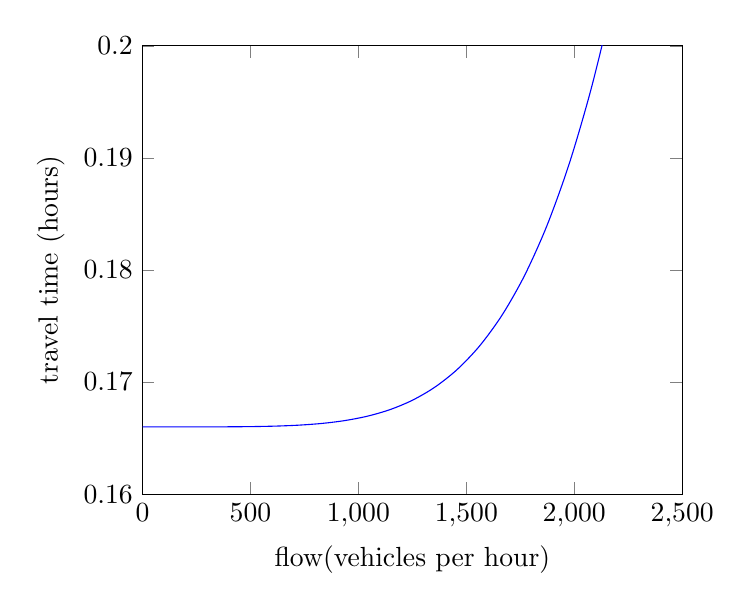
\begin{tikzpicture}
        \begin{axis}
            [
                domain=0:2500,
                black, no markers, smooth,
            %xtick=\empty, ytick=\empty,
                xlabel=flow(vehicles per hour), ylabel=travel time (hours),
                xmin=0,xmax=2500,
                ymin=0.16,ymax=0.2,
                yticklabel style={/pgf/number format/fixed, /pgf/number format/precision=3}
            ]
            \addplot {0.166*(1+0.15*(x/2000)^5)}; 
        \end{axis}
    \end{tikzpicture}
    \caption{Travel time function.}
    \label{fig:flowfunction}
\end{figure}
\todo{comment and correct graph}

Modifying Step 1 of the GSP for A* search:
\begin{algorithm}
    \caption{A* Search Algorithm}
    \begin{algorithmic}[1]
        \Procedure{AStar}{$s, t$}
        \State $\mathcal{Q} \gets \{s\}$ \Comment{Add node $s$ with $d_s = h_s$}
        \State $p_s \gets -1$
        \State $d_s \gets 0$
        \ForAll {$ u \in \mathcal{V} : u \neq s $} \Comment{All nodes unvisited except the source}
        \State $d_u \gets \infty$
    \EndFor

    \While{ $\mathcal{Q} \neq \emptyset$ }
    \State $ u \gets \text{top}(Q) $ \Comment{Remove $u$ such that $d_u + h_u = \displaystyle\min_{v \in \mathcal{Q}} \{ d_v + h_v \} $}
    \State $ \mathcal{Q} \gets \mathcal{Q} \char`\\ \{u\} $
    \If{ $u = t$ }
    \State \text{Terminate Procedure}
\EndIf
\If{ $u \neq \text{zone} $}
\ForAll {$v : (u, v) \in \mathcal{A}$} \Comment{For all successors of $u$}
\If {$d_u + c_{vw} < d_v$}
\State $d_v \gets d_u + c_{vw}$
\State $p_v \gets u$
                        %\If {$v \notin \mathcal{Q}$} \Comment{Include node $v$ if unvisited}
\State $\mathcal{Q} \gets \mathcal{Q} \cup \{v\}$ \Comment{Add node $v$ with $d_v = d_u + c_{vw} + h_v$}
                        %\EndIf
                    \EndIf
                \EndFor
            \EndIf
        \EndWhile
    \EndProcedure
\end{algorithmic}
\end{algorithm}
\todo[inline]{where are my $h$? heuristic?}


\begin{comment}
Comparing the Dijkstra and A* search algorithm's result,
we see an approximately 5 times improvement.
By looking at the shortest path tree generated
by the ChicagoSketch network,
there are only a few scanned nodes,
the path goes straight to the destination.
(TODO reference) says the closer the heuristic is to the actual distance,
the better/faster shortest path calculation,
by looking at the travel time function (Figure~\ref{fig:flowfunction}, we can see the slope
is really shallow near the start,
and by comparing the initial flow and final flow (TODO, data),
they are very close so the final flow is very close to the
initial flow,
which means the heuristic is a very good estimation,
which is our A* search is very fast.
\end{comment}

\section{Bidirectional A*}
\section{Preprocessing}

